I have tried various methods for estimating the position of the drone system
-- particularly with the goal of determining the velocity of the drone in order to remove the bouncing
that the DecaWave system exhibits.
I initially tested these sensors in isolation to determine which is the most viable,
and therefore where I should most apply my efforts.
It is especially important to note that indoor environments are quite variable,
and not all sensors are applicable to all environments.
In this section I explain the exploratory tests to determine which sensors are viable in V207,
and I discuss the possible factors influencing their behavior.

\subsection{Optical Flow}

The first sensor in the experiments is an ArkFlow optical flow sensor (See Figure~\ref{figure:arkflow_mount}),
which determines x/y-velocity using pixel velocity in a downward-facing camera.
This sensor is used in GPS-denied drone flight to extract velocity information from the
relative movement of the terrain beneath the drone.

\begin{figure}
	\centering
	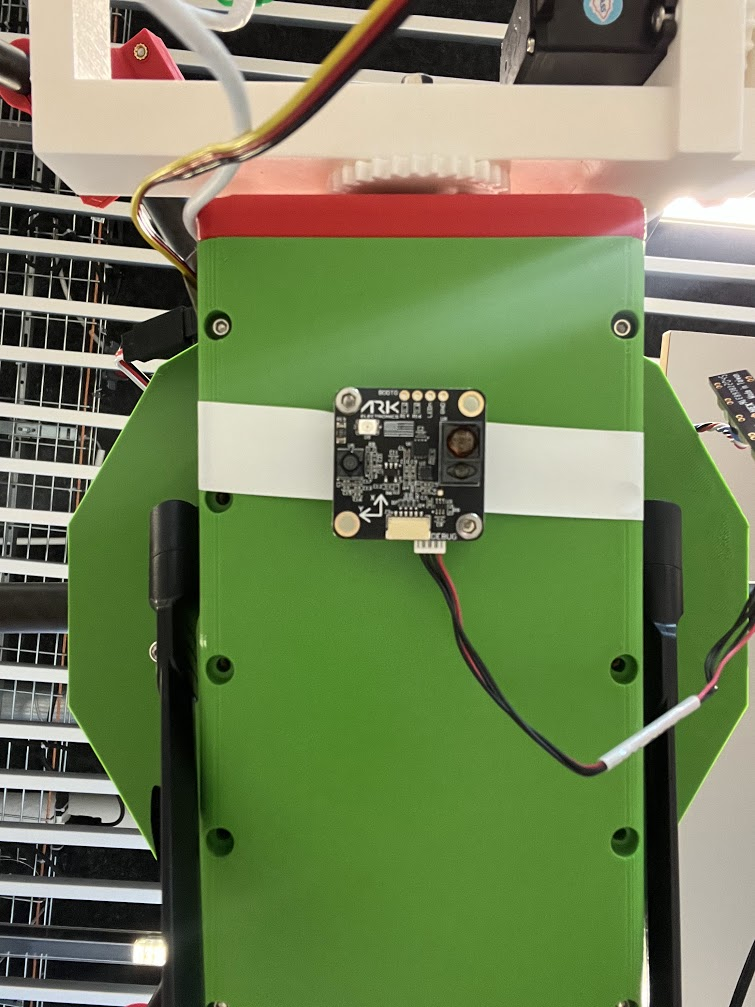
\includegraphics[width=0.5\linewidth]{./images/arkflow_mount}
	\caption{The ArkFlow sensor mounted to the bottom of the drone.}
	\label{figure:arkflow_mount}
\end{figure}

Initial tests show that the sensor is able to perceive motion from a pixel environment
with some variance.
Its raw data is also in some abstract form that must be processed by the flight controller unit (FCU)
before use.
Therefore, the velocity estimate from this sensor came from the FCU directly.
Ultimately, it also has difficulty determining its velocity from the very self-similar floor of V207.
Figure~\ref{figure:arkflow_performance_velocity} and~\ref{figure:arkflow_performance_position} show
the noisy velocity and position estimates respectively.
The velocity signal shows a sharp discontinuity in $t\in[65, 74]$,
and a large negative spike at $t=50$,
both of which do not correspond to the reality of the exploratory test.
These are made clearer by the position estimate in Figure~\ref{figure:arkflow_performance_position},
which essentially shows teleportation.
It is possible that this is not only due to the ArkFlow sensor, but also to the FCU's data fusion methods.
However, given time limitations, this method was not explored further.

\begin{figure}
	\centering
	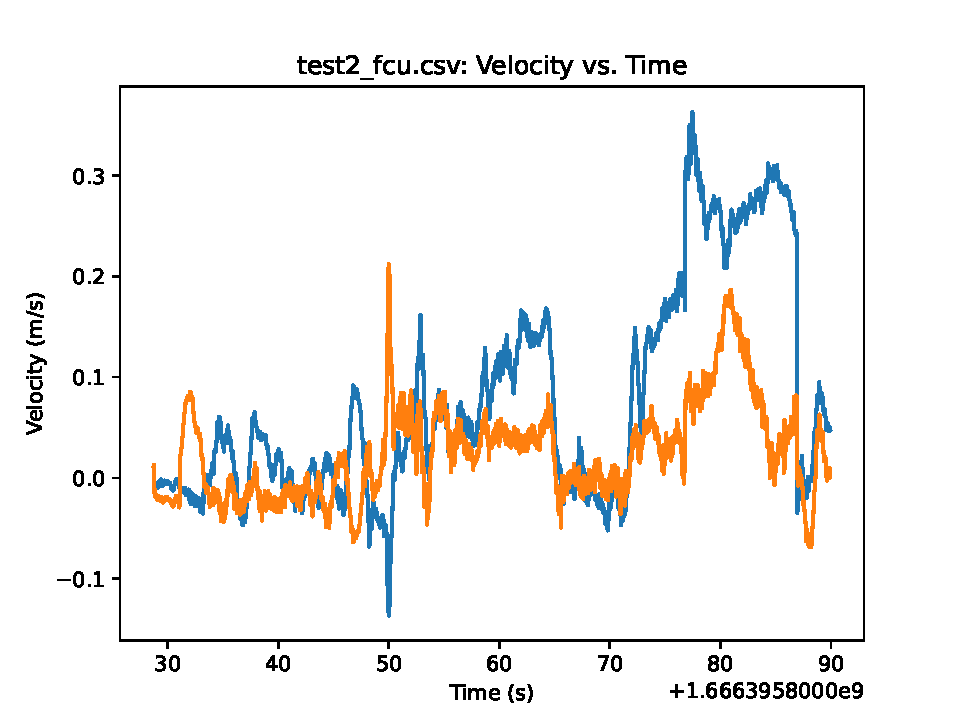
\includegraphics[width=\linewidth]{./images/test2_fcu_velocity}
	\caption{The velocity estimate from the FCU, fusing the ArkFlow data with IMU. Blue and orange correspond to the $x$ and $y$ dimensions respectively.}
	\label{figure:arkflow_performance_velocity}
\end{figure}

\begin{figure}
	\centering
	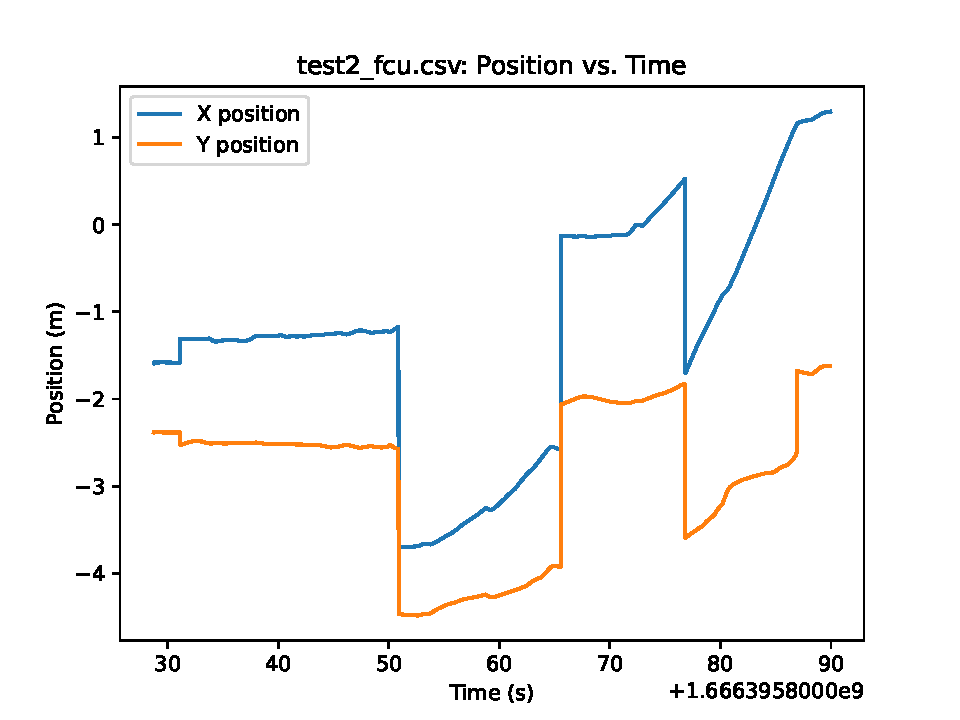
\includegraphics[width=\linewidth]{./images/test2_fcu_position}
	\caption{The position estimate from the FCU, fusing the ArkFlow data with IMU. Blue and orange correspond to the $x$ and $y$ dimensions respectively.}
	\label{figure:arkflow_performance_position}
\end{figure}

\subsection{Depth Flow}

A D455 stereo depth camera provides a relatively clean 3-dimensional view of the scene
in front of the drone.
Let $d_{r,i}$ represent the $i^\mathrm{th}$ \emph{raw} 640x480 depth image
generated from the D455 camera at index $i$.
This is referred to as \emph{raw} because its data is scalar multiples of some \texttt{depth\_scale} $s$
that is included as metadata, according to standard practices in the \texttt{pyrealsense2} library
that connects Python to the sensor itself.
We convert a \emph{raw} depth image $d_{r,i}$ to a depth image $d_i$ simply by multiplying the image
by the depth scale $s$ after converting it to a Numpy array.
So
$$d_i = d_{r,i} \cdot s$$
where $d_i$ is a \emph{depth image},
$d_{r,i}$ is a \emph{raw depth image},
and $s$ is a \emph{depth scale}.

Then, the velocity at index $i$ -- $v_i$ -- is as such:
$$v_i = \dfrac{d_i - d_{i-1}}{\Delta t}$$
where $t=t_i-t_{i-1}$ is the difference in timestamps between $d_i$ and $d_{i-1}$
At this point, the pixel position of the data is no longer important,
so I reshape the 2D array into a 1D array in order to operate on it more easily.

\begin{figure}[ht]
	\centering
	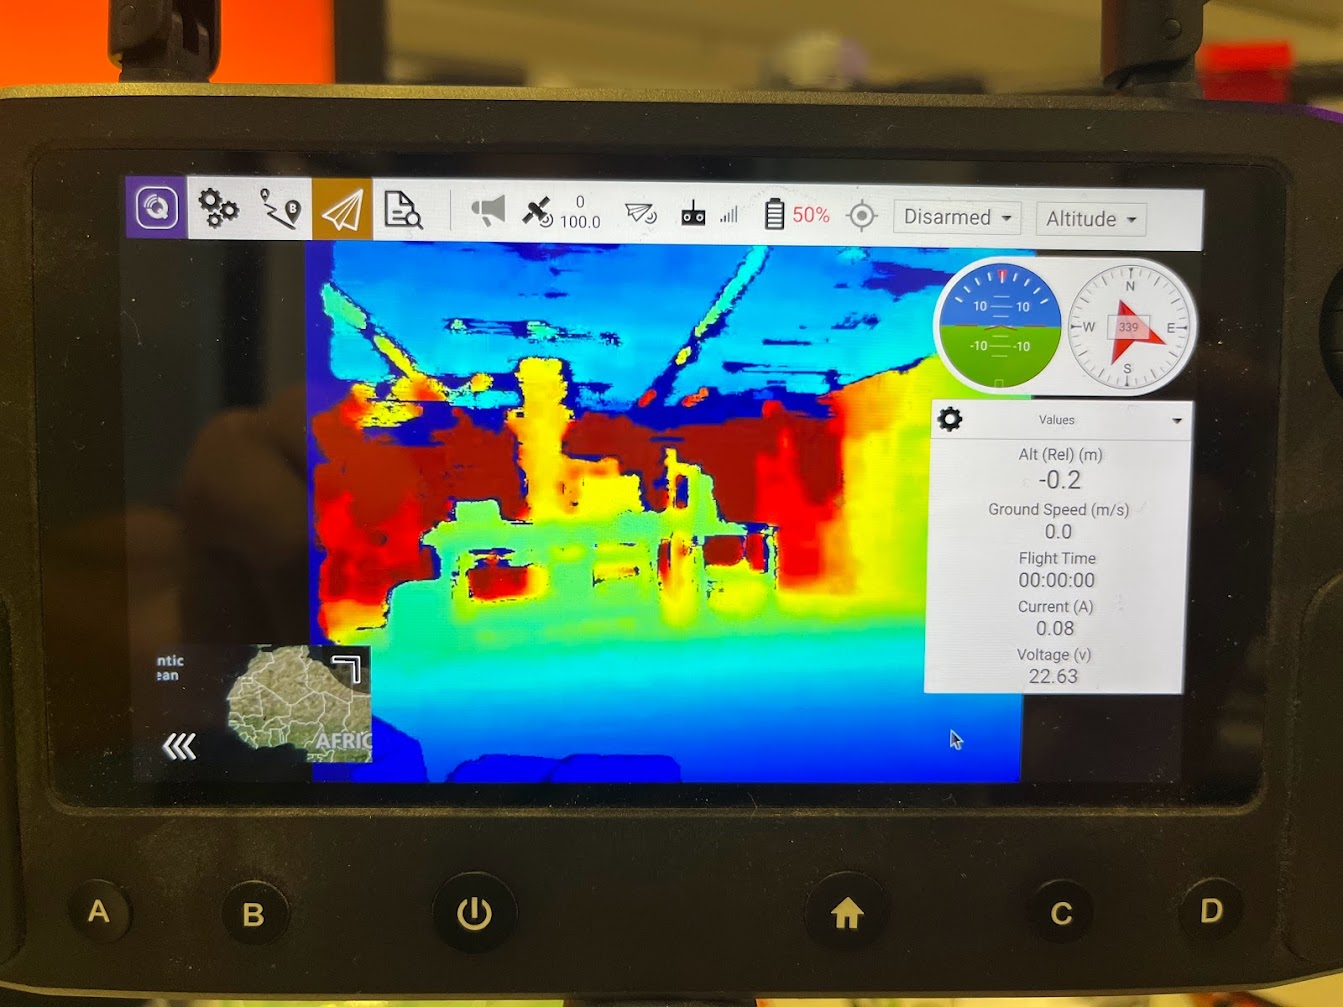
\includegraphics[width=0.6\textwidth]{./images/d455_sample.jpg}
	\caption{A sample image from the D455.}
	\label{figure:d455_sample}
\end{figure}
The edges around objects in the depth image are somewhat noisy and discontinuous,
as shown in Figure~\ref{figure:d455_sample},
and this can lead to high perceived pixel velocity in the depth dimension.
To remove this particular type of noise, I simply remove all velocity estimates
above a threshold of 1 m/s magnitude, decreasing the size of the velocity array $v_i$.
The whole velocity vector can then be aggregated into a single measurement using a simple arithmetic mean.

To test the overall performance, I recorded the aggregated velocity measurement over time
and plotted it for easy visualization.

For the first test, shown in Figure~\ref{figure:d455_velocity_still},
I simply left the drone still and recorded the velocity over time.
The plot shows relatively little noise -- less than 5 cm/s.
The second test, shown in Figure~\ref{figure:d455_velocity_quick} correctly depicts
discrete time segments of backwards and forwards motion and stillness.
This method of forward/backward velocity estimation appeared promising enough to use in later experiments.

\begin{figure}
	\centering
	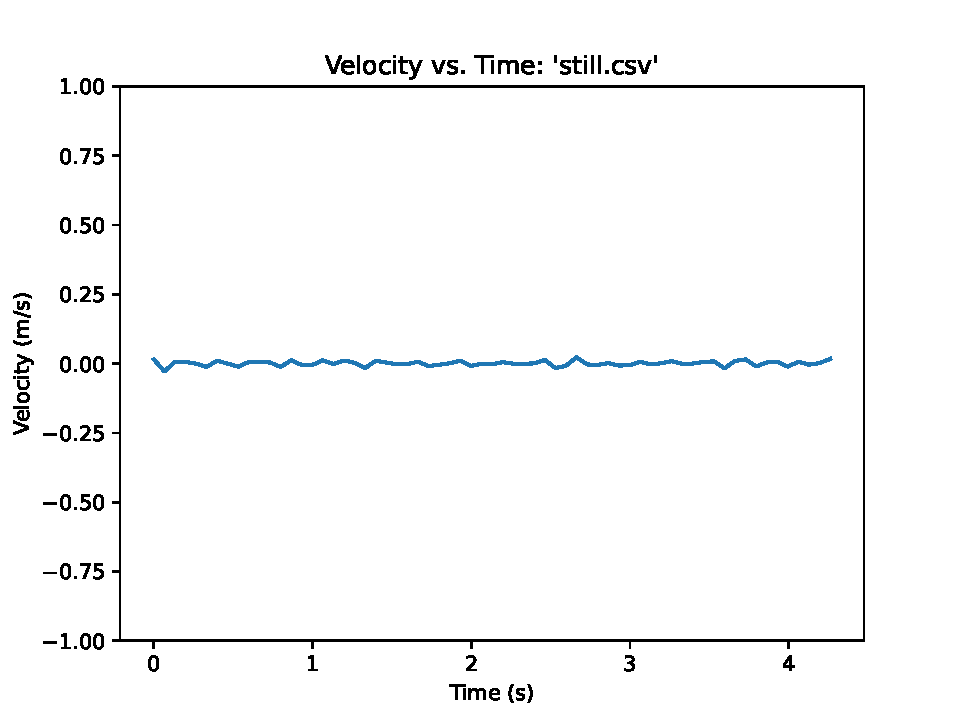
\includegraphics[width=\linewidth]{./images/still.pdf}
	\caption{The perceived velocity while the drone was sitting still.}
	\label{figure:d455_velocity_still}
\end{figure}

\begin{figure}
	\centering
	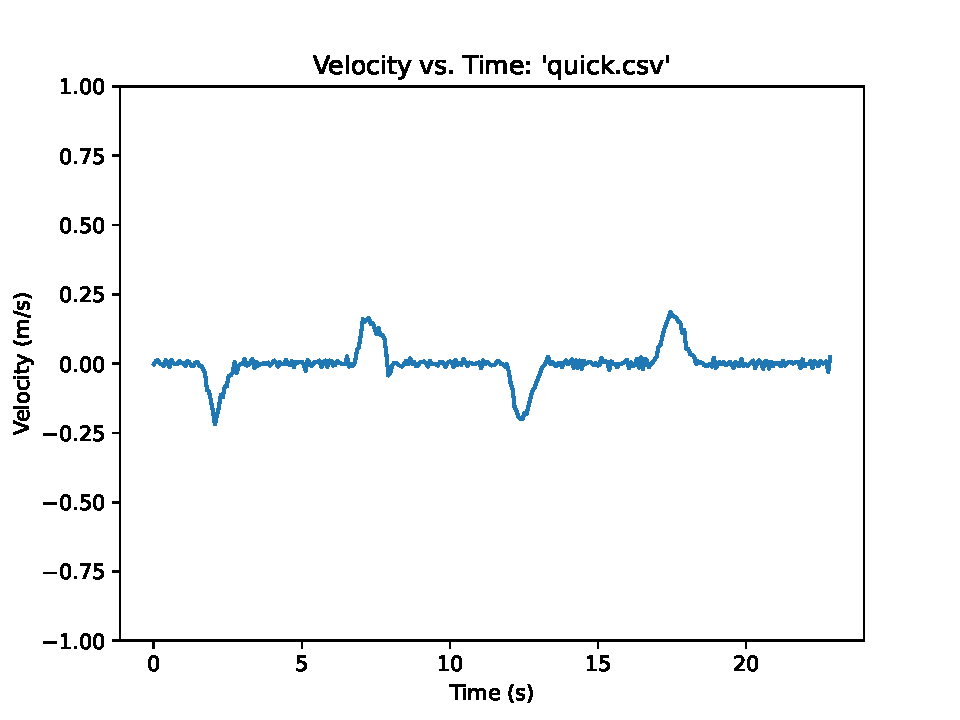
\includegraphics[width=\linewidth]{./images/quick.pdf}
	\caption{The perceived velocity while I moved the drone backwards and forwards quickly twice, leaving it still for a short time between movements.}
	\label{figure:d455_velocity_quick}
\end{figure}

\subsection{Heading Estimation}

The D455 has an inertial measurement unit with a gyroscope and accelerometer,
for estimation of angular velocity and orientation to the gravity vector.


\begin{figure}[h]
	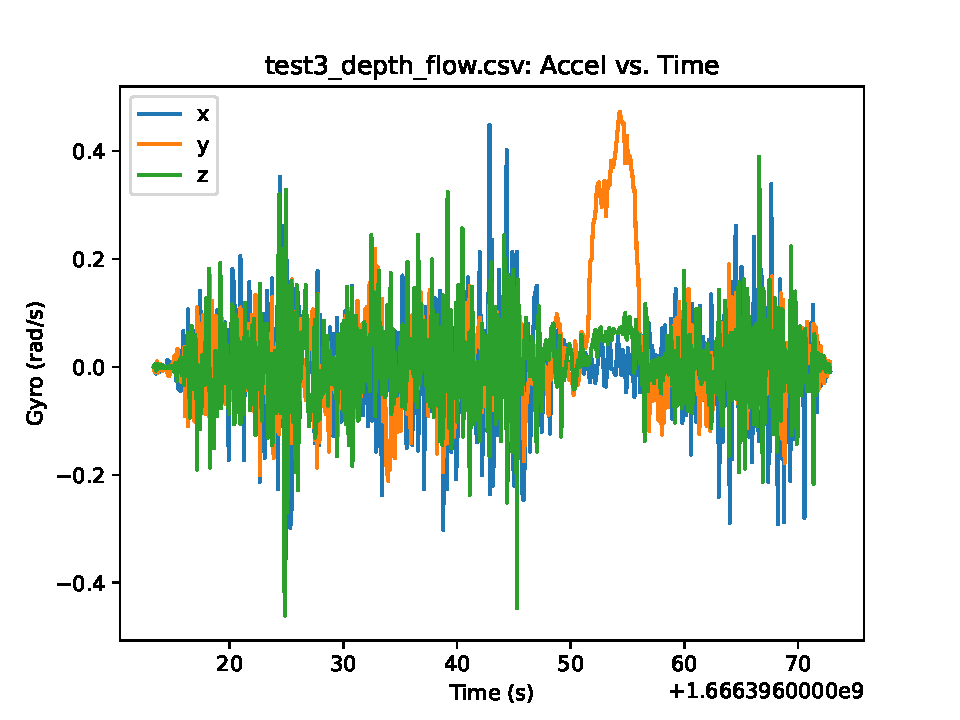
\includegraphics[width=\linewidth]{./images/test3_depth_flow_depth_gyro.pdf}
	\caption{A test of the gyroscope, showing a noise in $x$ and $z$ dimension,
	and a large, correct spike in the $y$ dimension which corresponds to a rotation of the drone
	in the yaw dimension.}
	\label{figure:test3_depth_gyro}
\end{figure}


